\documentclass{article}

\usepackage[a4paper, total={7in, 10in}]{geometry}

\usepackage{subcaption}
\usepackage{graphicx}
\usepackage{amssymb}
\usepackage{caption}
\usepackage{xcolor}
\usepackage{listings}
\usepackage{amsmath}
\usepackage{hyperref}
\usepackage{braket} 
\usepackage[spanish]{babel}

\usepackage[numbers]{natbib}
\bibliographystyle{plainnat}


\definecolor{carminered}{rgb}{1.0, 0.0, 0.22}
\definecolor{capri}{rgb}{0.0, 0.75, 1.0}
\definecolor{brightlavender}{rgb}{0.75, 0.58, 0.89}

\title{\textbf{Investigación Preliminar}}
\author{R.B. | I.B. | X.R. | A.M. | A.D. | J.P.R. \\ Dr. Iván Ongay}
\date{25 de Marzo, 2025}
\begin{document}

\pagecolor{black} 
\color{white}
\maketitle

\selectlanguage{spanish} 

\begin{abstract}
    Se condujo una breve investigación preliminar para identificar factores significativos cuyos tendrán un impacto notable a lo largo de el desarrollo de el proyecto en cuestión. 
\end{abstract}

\begin{Large}
\tableofcontents
\end{Large}%
\pagebreak

\section{Introducción} \label{sec:intro}
Pinchi investigación mamalona que nos aventamos alv

\section{Características de Mercado} \label{sec:caracmerc}
En esta sección exploramos algunas características de el mercado en cuestión (Emisiónes de tarjetas crediticias por Fintechs), para así, conocer algunos aspectos relevantes a el proyecto en desarrollo.

\subsection*{Resumen Rappicard}
RappiCard ha emergido como un actor significativo en el mercado mexicano de tarjetas de crédito desde su lanzamiento en 2021. A continuación, se presentan datos clave que ilustran su crecimiento y posición en el sector:

\begin{itemize}
    \item \textbf{Cartera de crédito:} Para agosto de 2024, RappiCard alcanzó una cartera de crédito de 5,107 millones de pesos, consolidándose entre las fintech más destacadas del país~\cite{forbes_cartera_2024}.
    \item \textbf{Número de clientes:} En abril de 2024, la empresa superó el millón de clientes en México, reflejando una rápida adopción de sus servicios \cite{expansion_millon_2024}.
    \item \textbf{Líneas de crédito:} Gracias al análisis de datos de la plataforma Rappi, RappiCard ofrece líneas de crédito iniciales promedio de $18,000$ MXN, un 53\% superiores a las de otras fintechs \cite{chocale_millon_2024}.
    \item \textbf{Segmento demográfico:} Aproximadamente el 75\% de los clientes de RappiCard tienen menos de 35 años, indicando un enfoque exitoso en atraer a la población joven y digitalmente activa \cite{expansion_millon_2024}.
    \item \textbf{Proceso de aprobación y entrega:} RappiCard se distingue por su proceso ágil, con aprobaciones en dos minutos y entrega de la tarjeta física en un promedio de 30 minutos en áreas con cobertura de Rappi \cite{forbes_cartera_2024}.
    \item \textbf{Beneficios adicionales:} La tarjeta ofrece recompensas como 5\% de cashback en compras a través de RappiTravel y 1\% en otros comercios, además de no cobrar anualidad y permitir diferir compras mayores a $500$ MXN a meses sin intereses \cite{chocale_millon_2024}.
    \item \textbf{Índice de Morosidad (IMOR) de Banorte:} En el informe financiero del cuarto trimestre de 2023, se reportó un incremento en el índice de morosidad (IMOR) del segmento de tarjetas de crédito de Banorte, alcanzando el 3.3\%. Este aumento se atribuye a la consolidación de Banorte con RappiCard, ya que el IMOR era de 2.4\% en el mismo período del año anterior. El IMOR es una métrica clave en el análisis de riesgo crediticio, que mide el porcentaje de clientes que no han realizado pagos en sus tarjetas de crédito dentro de los plazos establecidos \cite{fintechexpertrappicardmorosidad}.
    \item \textbf{Visión de José Antonio Murillo, CEO de RappiCard:} En cuanto al futuro de la alianza entre RappiCard y Banorte, José Antonio Murillo comentó: “Hay mercado para todos”. Esta declaración refleja la confianza de RappiCard en su modelo de negocio y en la demanda de servicios digitales en el sector financiero, especialmente ante el auge de las fintechs como la propia RappiCard \cite{forbesrappibanorte}.
    \item \textbf{Modelo de operación digital de RappiCard:} El CEO de RappiCard también destacó que su modelo de operación digital, combinado con atención personalizada, ha sido un factor clave para su éxito. RappiCard ha logrado un Net Promoter Score (NPS) superior a los 80 puntos, comparado con el promedio de 37 puntos en la banca tradicional según encuestas de Banxico. Esto indica que los usuarios están muy satisfechos con el servicio y están dispuestos a recomendarlo, lo que refuerza su posición en el mercado \cite{forbesrappibanorte}.
    \item \textbf{Crecimiento de RappiCard:} Desde su lanzamiento en enero de 2021, RappiCard ha emitido más de 700,000 tarjetas de crédito y cuenta con un portafolio de crédito que supera los 4,000 millones de pesos. A tan solo dos años de su entrada al mercado, RappiCard ya ha superado en emisión de tarjetas a bancos internacionales establecidos desde hace décadas, lo que destaca su rápido crecimiento y aceptación~\cite{forbesrappibanorte}.
\end{itemize}

Estos indicadores reflejan el crecimiento acelerado y la sólida posición de RappiCard en el mercado financiero mexicano, especialmente entre los consumidores jóvenes y familiarizados con la tecnología.

\vspace{0.3cm}

\begin{itemize}
    \item El ecosistema fintech en México creció a una tasa del 18\% anual entre 2019 y 2023~\cite{dock2024}.
    \item Existen 844 startups fintech activas en el país~\cite{finnovating2024}.
    \item En 2023, las fintechs otorgaron más de 3,000 millones de dólares en préstamos, beneficiando a más de 5 millones de usuarios~\cite{uflow2024}.
    \item En 2021, solo el 32.7\% de la población entre 18 y 70 años tenía al menos un crédito formal~\cite{inegi2021}.
    \item Los ingresos del sector fintech crecieron a una tasa compuesta del 22\% anual entre 2021 y 2024, y 31\% en el último periodo (2023-2024)~\cite{reporteindigo2024}.
    \item El Índice de Maduración del Ecosistema Fintech (INFIN) se sitúa en 48\%, indicando una etapa de desarrollo aún temprana~\cite{santander2024}.
    \item Solo el 20\% de la población mexicana tiene una tarjeta de crédito; el efectivo sigue siendo el medio de pago principal~\cite{elfinanciero2024}.
\end{itemize}

En conjunto, estos indicadores reflejan un sector en plena transformación, con un impacto creciente en el acceso al crédito y la inclusión financiera en México.

\begin{figure}[h!]
    \centering
    \begin{subfigure}[b]{0.45\textwidth} % 'h!' for positioning
        \centering
        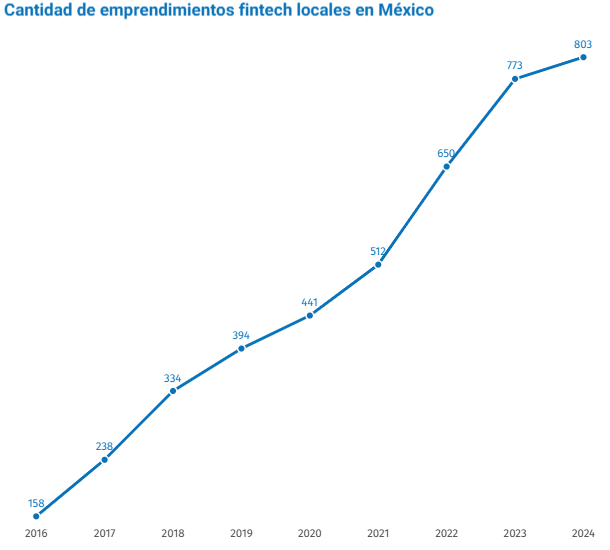
\includegraphics[scale=0.5]{Figuras/crecimientofintec.png} % scale the figure here
        \captionsetup{labelfont={color=white}, textfont={color=white}} % Cambia el color del caption
        \caption{Crecimiento de Fintechs.}
        \label{fig:crecfintechs}
    \end{subfigure}
    \hspace{0.005\textwidth} % Add some horizontal space between the subplots
    \begin{subfigure}[b]{0.45\textwidth} % 'h!' for positioning
        \centering
        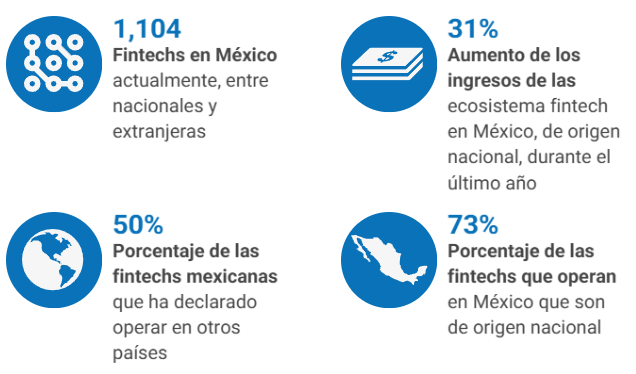
\includegraphics[scale=0.5]{Figuras/datosmercado.png} % scale the figure here
        \captionsetup{labelfont={color=white}, textfont={color=white}} % Cambia el color del caption
        \caption{Datos de Mercado.}
        \label{fig:datmerca}
    \end{subfigure}
    \captionsetup{labelfont={color=white}, textfont={color=white}} % Cambia el color del caption
    \caption{Fuente: Finnovista,  Fintech Radar México, 2025}
    \label{fig:figure1}
\end{figure}


\subsection*{Mercado: Tarjetas y Créditos}
De acuerdo con las bases de datos de la Comisión Nacional Bancaria y de Valores (CNBV)~\cite{cnbv_inclusion_2024}, se construyeron las siguientes tablas que se presentan a continuación.

\begin{table}[h!]
    \centering
    \caption{\textcolor{white}{Número de tarjetas de crédito por tipo de institución (trimestral)}}
    \color{white}
    \begin{tabular}{lcccccc}
        \hline
        \textbf{Institución} & \textbf{2023 T1} & \textbf{2023 T2} & \textbf{2023 T3} & \textbf{2023 T4} & \textbf{2024 T1} & \textbf{2024 T2} \\
        \hline
        Banca Múltiple       &        32,538,425         &        33,380,788         &       34,006,416          &       34,603,588          &        35,110,103         &        35,843,245    \\
        Banca de Desarrollo  &       20,362         &          20,495       &        20,680         &         20,601        &        20,756         &        21,037        \\
        Sofipos              &     3,487,589         &         3,155,757        &        4,011,168         &        3,427,085         &        3,955,533         &        5,194,963      \\
        Socaps               &       4,544          &           6,372      &       9,544          &         13,508        &        17,955         &            22,901     \\
        \hline
    \end{tabular}
    \label{tab:creditos_trimestrales}
\end{table}

\begin{table}[h!]
    \centering
    \caption{\textcolor{white}{Número total de créditos otorgados por tipo de institución (trimestral)}}
    \color{white}
    \begin{tabular}{lcccccc}
        \hline
        \textbf{Institución} & \textbf{2023 T1} & \textbf{2023 T2} & \textbf{2023 T3} & \textbf{2023 T4} & \textbf{2024 T1} & \textbf{2024 T2} \\
        \hline
        Banca Múltiple       &       59,480,857         &        60,704,810         &         61,731,925        &        62,709,348        &         63,108,527        &          64,949,134         \\
        Banca de Desarrollo  &       809,487        &        824,525         &         821,385         &         843,350         &         838,168        &           888,626         \\
        Sofipos              &        3,911,704          &          3,719,181       &         4,677,062          &         4,223,454        &        4,953,483         &           5,852,773       \\
        Socaps               &        2,814,646        &        2,852,568         &        2,861,541         &         2,844,703       &        2,830,927         &           2,898,419       \\
        \hline
    \end{tabular}
    \label{tab:total_creditos_trimestrales}
\end{table}

%% Estaria fino comparar esto contra dinero activo en el mercado i.e. total de dinero en mercado de credito (general; comparar contra \# tarjetas de credito) vs. total de dinero en el mercado de credito (fintech; comparar contra \# tarjetas de fintechs).

\subsection*{Población: Jóvenes $\in[18,30]$}

\subsection*{Población: Económicamente activos}

\subsection*{Hábitos de consumo (México)}

\subsection*{Población: Lineas telefonicas (no prepago)}

\subsection*{Población: Personas que cumplen con req. de ingresos}

\section{Forecast} \label{sec:forecasting}
Predecir valores futuros usando datos del pasado —lo que llamamos \textit{forecasting de series de tiempo}— es algo clave en muchas áreas como economía o negocios. En el caso de RappiCard, por ejemplo, saber cuántas tarjetas de crédito se necesitarán en el futuro ayuda a tomar mejores decisiones sobre cuántas producir y cuándo hacerlo.

Normalmente, este tipo de predicciones se hace con modelos estadísticos como ARIMA o modelos de machine learning como LSTM. Pero en este proyecto queremos probar algo distinto:

\textbf{Un modelo basado en geometría}, llamado \textit{Geometrical Realization for Time Series Forecasting} \cite{bayeh2024gr}.

Este modelo funciona de otra manera: en lugar de ver la serie de tiempo como una simple lista de números, la convierte en una especie de “figura” o “curva” en un espacio de más dimensiones. Luego, sobre esa figura aplica una transformación que permite hacer la predicción. El objetivo de esta sección es explicar bien cómo funciona ese enfoque y por qué creemos que tiene potencial para este proyecto. Ademas de la implementacion de este modelo, se ha decidido implementar un modelo estadistico, de esta manera se genera una comparacion entre dos prespectivas distintas de forecasting.

\subsection*{¿Qué es una \texttbf{serie de tiempo}?}
Una serie de tiempo es una colección de observaciones tomadas en momentos consecutivos, a intervalos regulares. Por ejemplo, el número de tarjetas emitidas por RappiCard cada trimestre es una serie de tiempo univariada. En general, las series pueden ser:

\begin{itemize}
    \item \textbf{Univariadas:} una sola variable (e.g. ventas mensuales).
    \item \textbf{Multivariadas:} varias variables relacionadas medidas en paralelo (e.g. ventas + gasto en marketing).
\end{itemize}

\subsection*{Preliminares al modelaje geométrico}

Antes de implementar modelos geométricos sobre una serie de tiempo, es necesario transformar esta serie en una estructura que capture su evolución temporal. A este proceso se le conoce como \textbf{embedding}, y es la piedra angular del enfoque propuesto en el artículo \textit{Geometrical Realization for Time Series Forecasting} \cite{bayeh2024gr}.

\subsubsection*{Delay Embedding}

Dado un conjunto de observaciones $x_1, x_2, \dots, x_n$ de una serie temporal univariada, se define el \textit{embedding de dimensión $d$ y retardo $\tau$} como la colección de vectores:
\[
\mathbf{x}^{(i)} = [x_i, x_{i-\tau}, x_{i - 2\tau}, \dots, x_{i - (d-1)\tau}]
\]
para $i$ tal que todos los índices sean positivos (es decir, $i \geq (d-1)\tau$).

Este procedimiento transforma la serie original en una secuencia de puntos en $\mathbb{R}^d$, permitiendo así analizar su comportamiento como una \textbf{curva} o \textbf{superficie} en un espacio de dimensión superior. Esta idea está inspirada en el \textbf{Teorema de Takens}, el cual garantiza (bajo ciertas condiciones) que esta transformación preserva las propiedades dinámicas del sistema original.

\paragraph{Ejemplo de Embedding:} Supongamos que tenemos la serie:
\[
[5, 8, 12, 18, 25, 35]
\]
Si usamos $d = 3$ y $\tau = 1$, el embedding produce:
\[
[ [12, 8, 5], [18, 12, 8], [25, 18, 12], [35, 25, 18] ]
\]
Cada uno de estos vectores puede verse como un punto en $\mathbb{R}^3$.

\subsubsection*{HD-Embedding (High-Dimensional Embedding)}

El embedding tradicional puede ser limitado si la serie no tiene una dinámica demasiado compleja. Sin embargo, cuando se desea capturar comportamientos no lineales y patrones más sutiles, se puede aumentar la dimensión $d$ y ajustar el retardo $\tau$ estratégicamente. A este proceso se le conoce como \textbf{embedding de alta dimensión (HD-Embedding)}.

La idea detrás del HD-Embedding es que, al representar los datos en un espacio más rico, se facilita el aprendizaje de estructuras geométricas subyacentes (como curvas o superficies algebraicas) que pueden capturar las reglas implícitas de evolución temporal.

Esta técnica es la base para los modelos implementados en los scripts que se presentan a continuación.

\subsection*{Modelo \texttt{polynomial\_model.py}}

Este modelo implementa una aproximación algebraica a la serie embebida. El objetivo es ajustar una función polinomial multivariada sobre los puntos del embedding para luego predecir valores futuros. A continuación se explica su funcionamiento:

\paragraph{1. \texttt{build\_polynomial\_model(degree, alpha):}} Esta función construye un pipeline de \texttt{scikit-learn} compuesto por:

\begin{itemize}
    \item \texttt{StandardScaler()}: Estandariza los datos.
    \item \texttt{PolynomialFeatures(degree)}: Genera todas las combinaciones polinomiales de las variables hasta el grado especificado.
    \item \texttt{Ridge(alpha)}: Aplica una regresión Ridge (con penalización L2) para evitar sobreajuste.
\end{itemize}

\paragraph{2. \texttt{fit\_model(X, y, degree, alpha):}} Ajusta el modelo sobre el conjunto de entrenamiento. Aquí:
\begin{itemize}
    \item \( X \in \mathbb{R}^{m \times d} \): puntos del embedding.
    \item \( y \in \mathbb{R}^m \): valores futuros a predecir (típicamente, el siguiente valor en la serie original).
\end{itemize}

\paragraph{3. \texttt{predict(model, x):}} Predice el siguiente valor en la serie, dado un vector de embedding.

\paragraph{4. \texttt{predict\_recursive(model, init\_point, steps):}} Realiza predicciones a múltiples pasos en el futuro. Usa la predicción anterior como entrada para la siguiente, imitando una simulación del sistema dinámico.

\paragraph{5. \texttt{search\_best\_degree\_alpha}:} Prueba múltiples combinaciones de grado polinomial y parámetros de regularización y selecciona la que minimiza el \textit{sMAPE} (symmetric Mean Absolute Percentage Error), útil para comparar rendimiento entre modelos con diferente escala.

\paragraph{Visualización:} Se genera un gráfico 3D del embedding original y otro con los puntos predichos. Se usa color y conectividad para mostrar claramente la evolución temporal y cómo la predicción se alinea (o no) con el embedding real.

\subsection*{Modelo \texttt{geo\_realization.py}}

Este script implementa una lógica distinta: en vez de ajustar un modelo simple sobre el embedding, construye una \textbf{superficie polinomial} sobre el embedding completo, tratando de parametrizarlo globalmente.

\paragraph{1. \texttt{fit\_surface\_to\_embedding(X, degree):}} Ajusta una superficie polinomial en $\mathbb{R}^3$ sobre los puntos del embedding. Internamente:
\begin{itemize}
    \item Se usa \texttt{PolynomialFeatures} para transformar los datos.
    \item Se ajusta un modelo \texttt{LinearRegression} (sin regularización) sobre el embedding para predecir la tercera coordenada a partir de las dos primeras.
    \item El resultado es una "variedad" (una especie de superficie algebraica) que intersecta todos los puntos del embedding.
\end{itemize}

\paragraph{2. \texttt{predecir\_desde\_superficie(punto\_actual, model):}} A partir de un nuevo punto $(x_0, x_1)$ del embedding, genera la coordenada $x_2$ usando la superficie ajustada. Esta es la lógica de predicción: buscar puntos en el embedding que sigan la dinámica estimada.

\paragraph{3. \texttt{predecir\_n\_puntos(X, model, n):}} Predice $n$ puntos futuros a partir del último punto en el embedding original. Cada nuevo punto predicho se vuelve entrada para el siguiente paso.

\paragraph{4. \texttt{plot\_embedding\_with\_surface(X, model, puntos\_predichos=None):}} Visualiza:
\begin{itemize}
    \item El embedding original (línea verde).
    \item La superficie ajustada (malla azul translúcida).
    \item Opcionalmente, los puntos predichos (línea roja).
\end{itemize}
Esto permite ver si los puntos futuros siguen la forma del embedding o se desvían.

\paragraph{5. \texttt{evaluar\_modelo\_fragmentado(X, idx\_start, idx\_end):}} Permite seleccionar un fragmento del embedding para ajustar la superficie y evaluar predicciones hacia adelante y hacia atrás. Se reportan métricas como MAE y MSE entre los puntos predichos y los reales no usados en el entrenamiento.

Esta lógica nos permite evaluar si la superficie está capturando correctamente la forma global del embedding, incluso más allá del rango de datos usados para el ajuste. Es una herramienta que nos ayuda a entender si el modelo generaliza bien o si está sobreajustado.


\section{Optimización} \label{sec:optimiz}
\subsection*{Entendiendo: ¿Qué es un \textit{stock} en tarjetas de crédito?}

El objetivo es predecir cuántas tarjetas físicas (aún no activadas) deben fabricarse en cada periodo. Para esto, debemos tener en cuenta tres factores fundamentales:

\begin{enumerate}
	\item \textbf{Tarjetas físicas sin activar:} Son los objetos físicos que se deben tener listos para satisfacer la demanda futura. Su producción debe anticiparse al uso, pero sin caer en el exceso.
	
	\item \textbf{Demanda proyectada:} Depende de múltiples variables, como campañas de marketing (e.g. tarjetas temáticas), comportamiento regional y perfil de los usuarios (por edad, ingresos, historial).
	
	\item \textbf{Costos de sobreproducción o desabasto:} Sirven como función objetivo en la optimización. También se deben considerar costos de almacenamiento, distribución y tiempos de entrega.
\end{enumerate}

Esto nos lleva naturalmente a un problema de optimización bajo incertidumbre, con un componente predictivo fuerte (forecast) y decisiones estructurales que se prestan al modelado matemático.


\bibliography{biblio} 

\end{document}